\begin{figure}[ht]
  \centering
  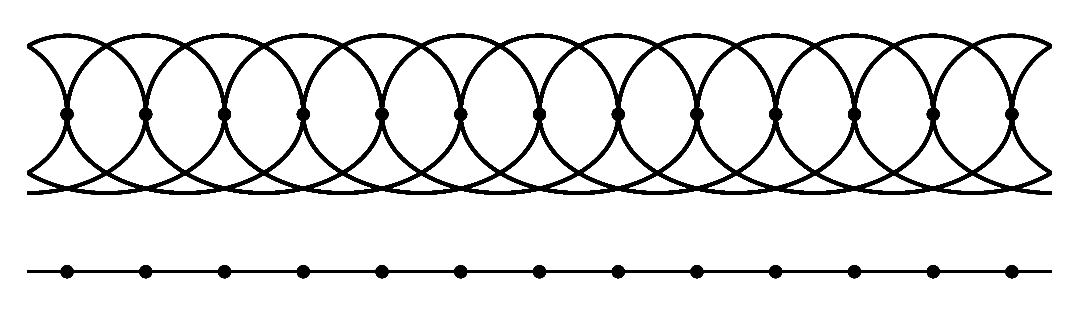
\begin{tikzpicture}
    \begin{scope}
    \clip (-6.5,-0.2) rectangle (6.5,3.1);

    \foreach \x in {-6,-5,...,6}{% Two indices running over each
      \foreach \y in {-6,-5,...,6}{% node on the grid we have drawn 
        \draw[line width=1pt](\x-1,0)--(\x+1,0);
        \node[draw,circle,inner sep=1.5pt,fill] at (\x,0) {};
            % Places a dot at those points
      }
    }
    
    \foreach \x in {-6,-5,...,6}{% Two indices running over each
      \foreach \y in {-6,-5,...,6}{% node on the grid we have drawn 
        \node[draw,circle,inner sep=1.5pt,fill] at (\x,2) {};
        \draw[very thick] (\x,2) arc[start angle=0, end angle=180, x radius= 1, y radius = 1];
        \draw[very thick] (\x+2,2) arc[start angle=0, end angle=180, x radius= 1, y radius = 1];
            
        \draw[very thick] (\x,2) arc[start angle=0, end angle=-180, x radius= 1.5, y radius = 1];
        \draw[very thick] (\x+3,2) arc[start angle=0, end angle=-180, x radius= 1.5, y radius = 1];
      }
    }
    \end{scope} 
  \end{tikzpicture}
  \caption{Dois espaços dentre os quais é possível traçar uma quasi-isometria.}
  \label{figure:cay(Z)}
\end{figure}